\newif\ifvimbug
\vimbugfalse

\ifvimbug
\begin{document}
\fi

\exercise{Principal Component Analysis}
In this exercise, you will use the dataset \texttt{iris.txt}. It contains data from three kind of Iris flowers (`Setosa', `Versicolour' and `Virginica') with 4 attributes: sepal length, sepal width, petal length, and petal width. Each row contains a sample while the last attribute is the label ($0$ means that the sample comes from a `Setosa' plant, $1$ from a `Versicolour' and $2$ from `Virginica').
(You are allowed to use built-in functions for computing the mean, the covariance, eigenvalues and eigenvectors.)

\begin{questions}

%----------------------------------------------

\begin{question}{Data Normalization}{3}
Normalizing the data is a common practice in machine learning. Normalize the provided dataset such that it has zero mean and unit variance per dimension. Why is normalizing important?
Attach a snippet of your code. 

\begin{answer}
In machine learning some methods like PCA take the variance of the features as a criterion for dimensionality reduction. If the feature differ in their range, the means and the variances of the features will have a different scale. To achieve better comparability among the features it is common to normalize the data to unit variance and zero mean. The normalization can be achieved by applying the following formula to all datapoints $x_i$ for each feature separately:
\begin{equation*}
\frac{x_i-mean_{feature}}{standard\_deviation_{feature}}
\end{equation*}
We calculated the means of the features as follows:
$$means=\begin{bmatrix} 
5.84333333 & 3.054 & 3.75866667 &1.19866667
\end{bmatrix}$$
We calculated the standard deviation of the features as follows:
$$standard\_deviation=\begin{bmatrix} 
0.82530129 & 0.43214658 & 1.75852918 & 0.76061262
\end{bmatrix}$$
We apply the normalization to the dataset according to the following code snippet.\\
\lstinputlisting[language=Python]{code/PCA_normalize.py}
\end{answer}

\end{question}

%----------------------------------------------

\begin{question}{Principal Component Analysis}{8}
Apply PCA on your normalized dataset and generate a plot showing the proportion (percentage) of the cumulative variance explained. 
How many components do you need in order to explain at least $95\%$ of the dataset variance? 
Attach a snippet of your code.
\begin{answer}
For doing the PCA, after normalizing, we have to compute the covariance matrix and subsequently calculate the eigenvectors and eigenvalues of the covariance matrix.\\
As Figure \ref{fig:1} shows, by using two principal components we can explain 95,8\% of the cumulative variance. The four bars are calculated by using the following formula, whereas the eigenvalues are sorted from the biggest eigenvalue to the smallest eigenvalues:
\begin{equation*}
\textrm{proportion of cumulative variance explained by n biggest eigenvectors} = \frac{\textrm{sum of n biggest eigenvalues}} {\textrm{sum of all eigenvalues}} 
\end{equation*}
For the covariance matrix of the normalized data we obtain:
$$\Sigma=\begin{bmatrix} 
1.00671141 & -0.11010327 & 0.87760486 & 0.82344326 \\
-0.11010327 & 1.00671141& -0.42333835& -0.358937  \\
0.87760486 &-0.42333835 & 1.00671141 & 0.96921855 \\
0.82344326& -0.358937  &  0.96921855 & 1.00671141
\end{bmatrix}$$
The eigenvalues have the following values:
$$eigenvalues = \begin{bmatrix} 
2.93035378 & 0.92740362& 0.14834223 &0.02074601
\end{bmatrix}$$
The eigenvectors have the following values. The eigenvectors are sorted according to their respective eigenvalues above. Each column contains one eigenvector.
$$eigenvectors = \begin{bmatrix} 
 0.52237162 &-0.37231836 &-0.72101681 & 0.26199559\\
 -0.26335492 &-0.92555649 & 0.24203288 &-0.12413481\\
 0.58125401 &-0.02109478&  0.14089226 &-0.80115427\\
 0.56561105& -0.06541577 & 0.6338014 &  0.52354627
\end{bmatrix}$$
The following code snippet shows the code for doing the PCA and for plotting.\\
\lstinputlisting[language=Python]{code/PCA_explained_variance.py}
\end{answer}
\begin{figure}[h!]
	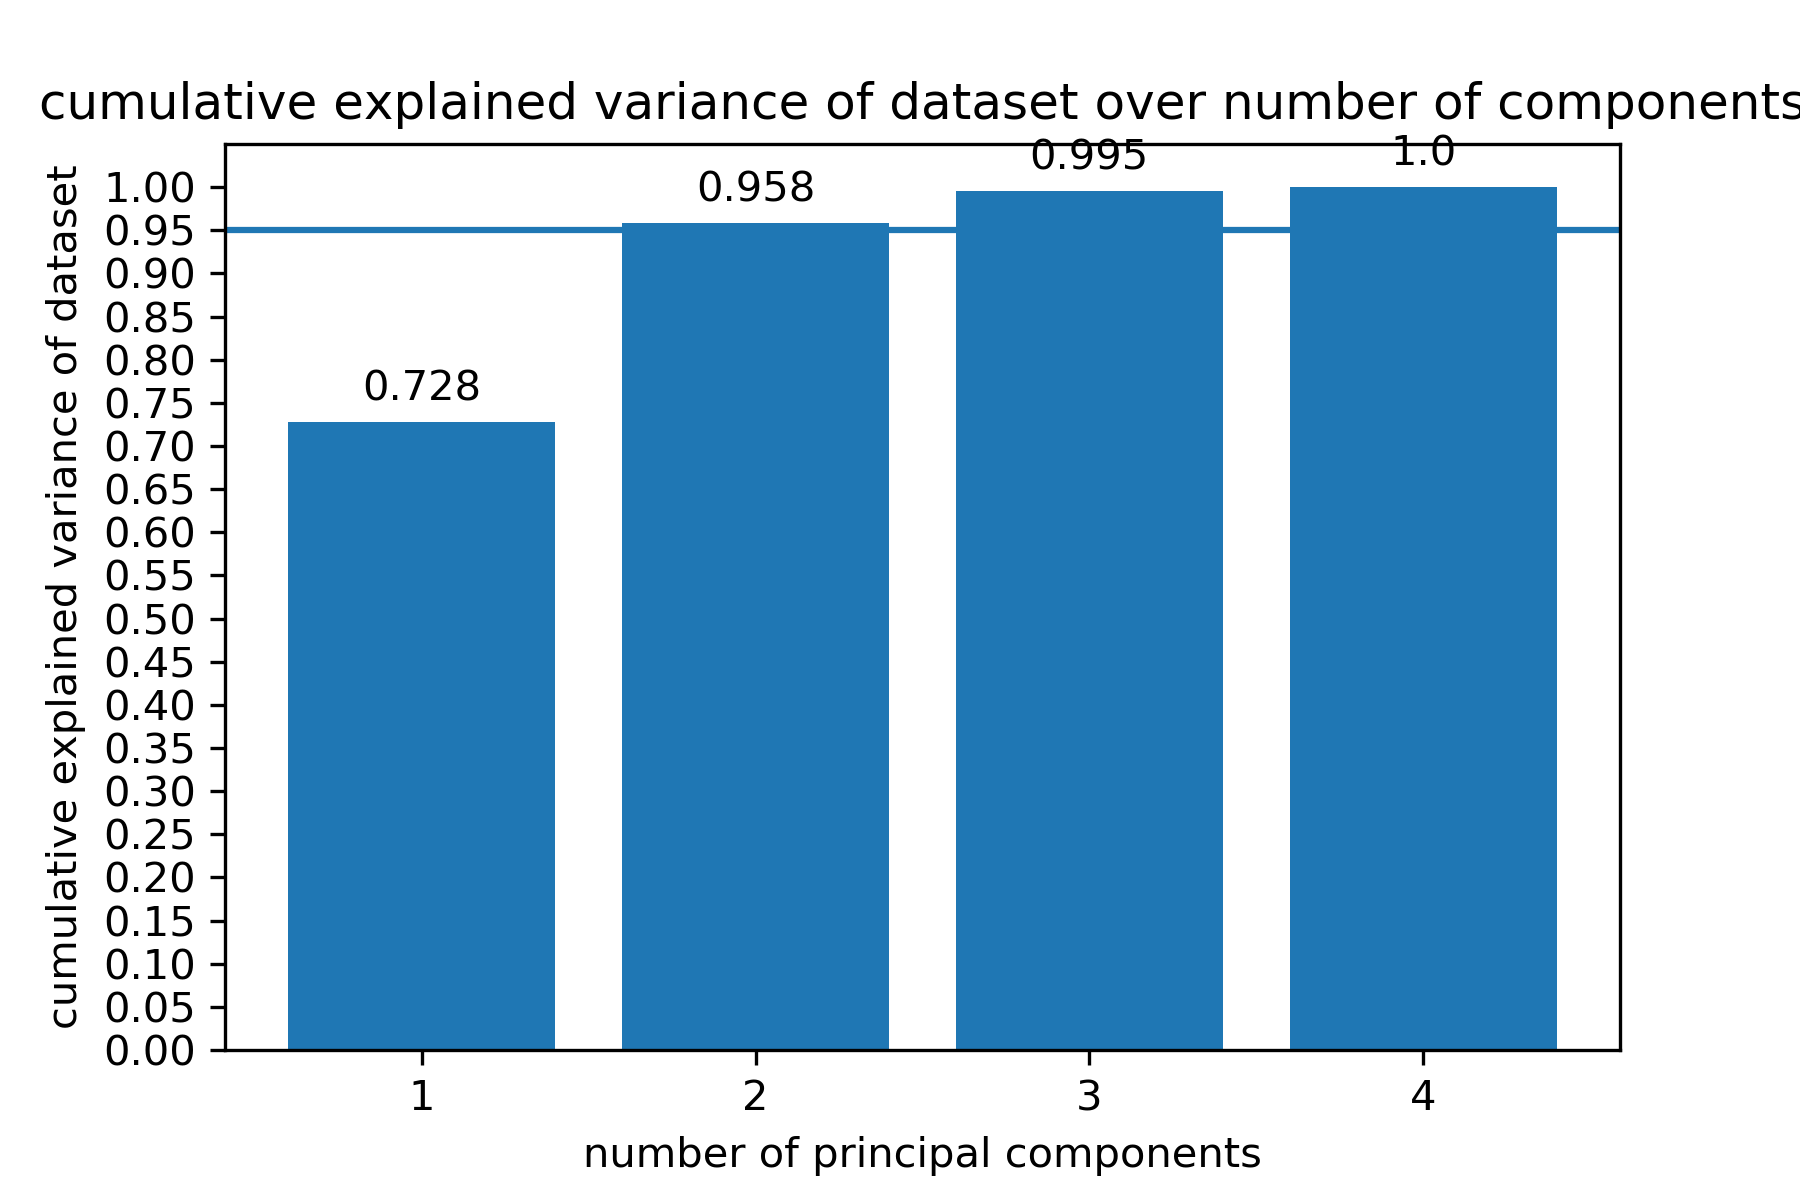
\includegraphics[width=0.8\linewidth]{pictures/explained_var_cumulative.png}
	\centering
	\caption{Cumulative explained variance of dataset over number of principal components.}
	\label{fig:1}
\end{figure}
\end{question}

%----------------------------------------------

\begin{question}{Low Dimensional Space}{6}
Using as many components as needed to explain $95\%$ of the dataset variance, generate a scatter plot of the lower-dimensional projection of the data. Use different colors or symbols for data points from different classes. 
What do you observe? Attach a snippet of your code.
\begin{answer}
For projecting the data to the lower dimensional space we use the following formula on the normalized dataset:
\begin{equation}
\mathbf{a}^{n}=\mathbf{B}^{\top}\mathbf{x}^{n}
\end{equation}
$\mathbf{a}^{n}$ is the projected data, $\mathbf{B}$ is a matrix containing the eigenvectors - in our case the two eigenvectors corresponding to the two biggest eigenvalues, for obtaining 2-dimensional projection - and $\mathbf{x}^{n}$ is the projected data. The two biggest eigenvalues with corresponding eigenvectors are:
$$eigenvalues =\begin{bmatrix} 
2.93035378 & 0.92740362
\end{bmatrix}$$
The eigenvectors have the following values. The eigenvectors are sorted according to their respective eigenvalues above. Each column contains one eigenvector.
$$eigenvectors = \begin{bmatrix} 
 0.52237162 &-0.37231836 \\
 -0.26335492 &-0.92555649 \\
 0.58125401 &-0.02109478\\
 0.56561105& -0.06541577 
\end{bmatrix}$$
The 2-dimensional projection leads to the scatter plot in Figure \ref{fig:2}. \\
We can observe that the Versicolour class is clearly separated from the Setosa and Verginica classes in the two-dimensional space. Between the Setoas and the Viriginica class, there is some overlapping, but the class means and variances are still different from each other. Since the two-dimensional projection contains over 95\% of the variance of the unprojected dataset, these results can be transferred to the unprojected dataset, too.\\
Building upon the previously used code, we have used the following code for the two-dimensional projection and the scatter plot.\\
\lstinputlisting[language=Python]{code/PCA_scatter.py}
\end{answer}
\begin{figure}[h!]
	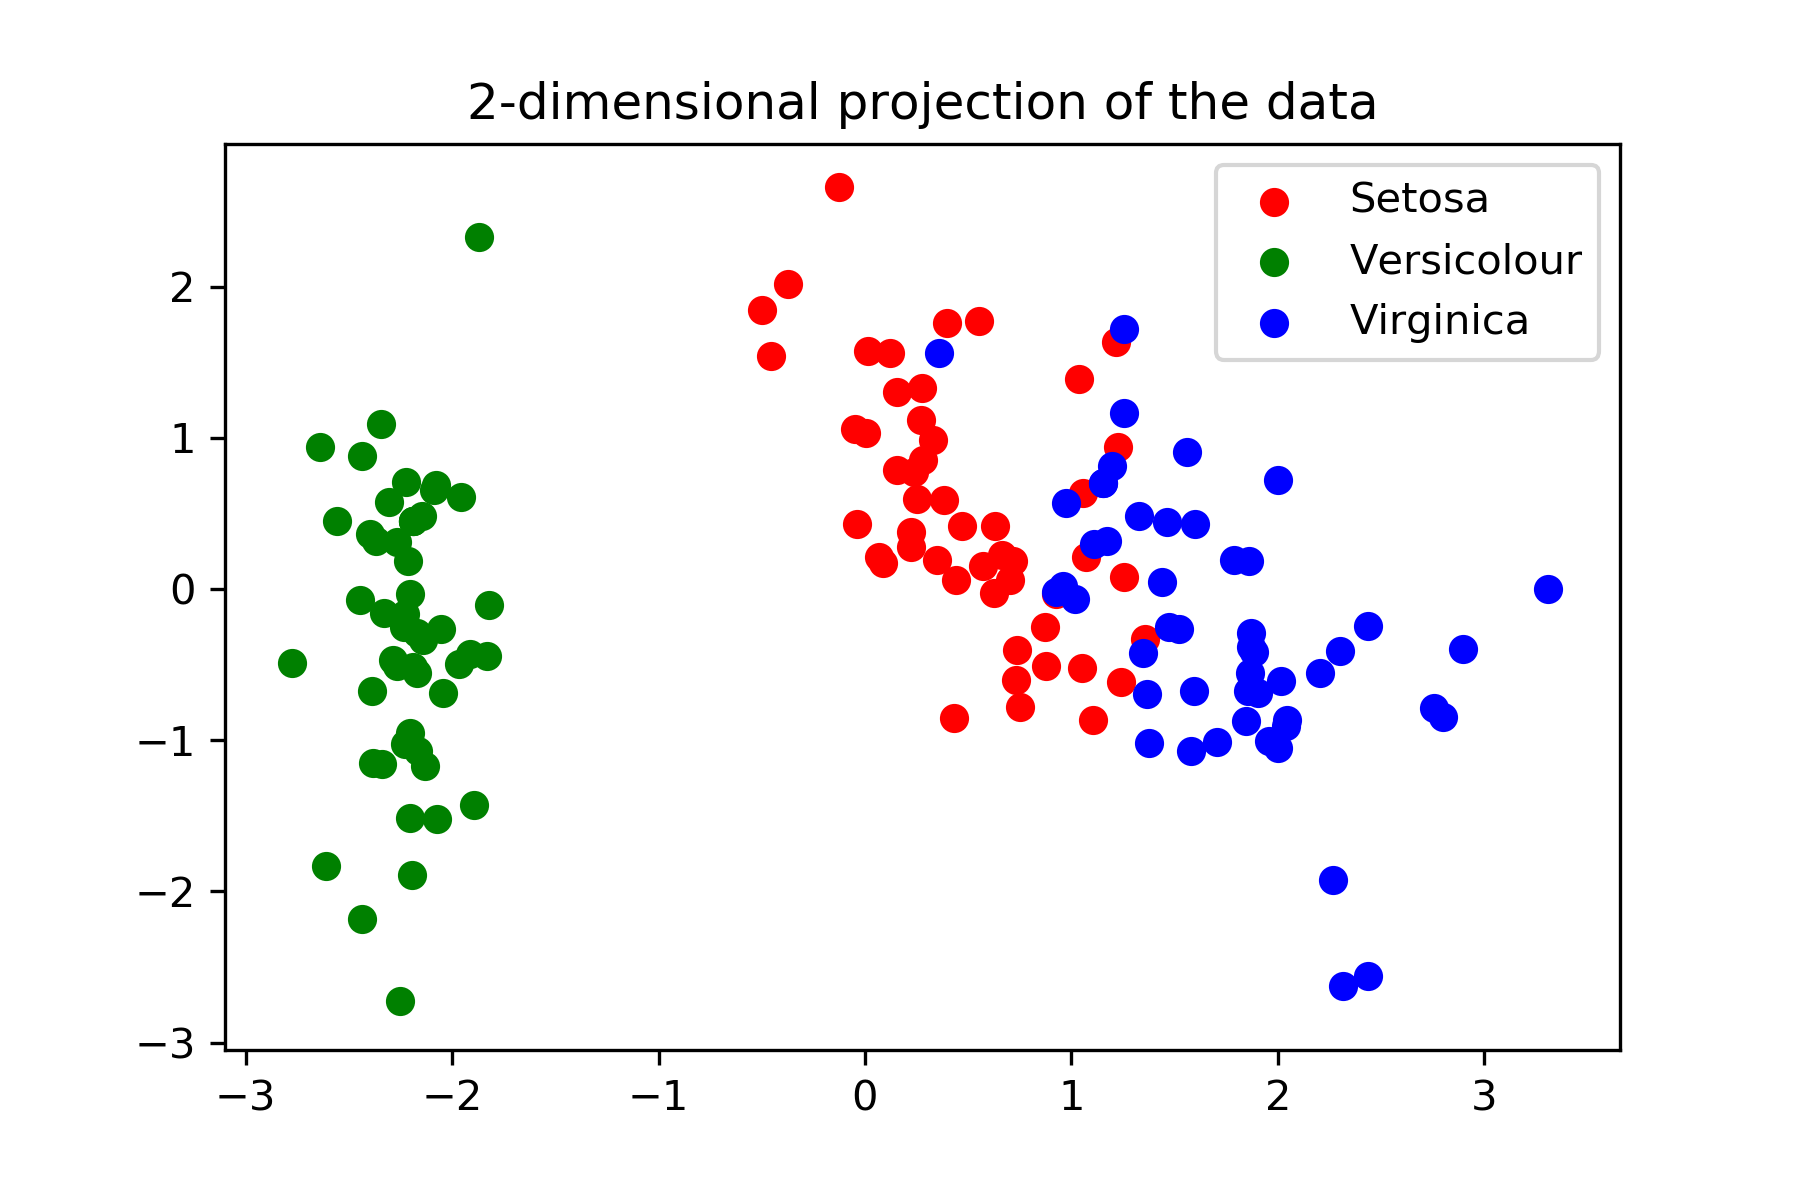
\includegraphics[width=0.8\linewidth]{pictures/PCA_scatter.png}
	\centering
	\caption{Scatter plot of the 2-dimensional projection of the data.}
	\label{fig:2}
\end{figure}
\end{question}

%----------------------------------------------

\begin{question}{Projection to the Original Space}{6}
Reconstruct the original dataset by using different number of principal components. Using the normalized root mean square error (NRMSE) as a metric, fill the table below (error per input versus the amount of principal components used).

\begin{tabular}{c|r|r|r|r}
N. of components & $x_1$ & $x_2$ & $x_3$ & $x_4$ \\
\hline
1 & & & & \\
2 & & & & \\
3 & & & & \\
4 & & & &
\end{tabular}

Attach a snippet of your code.
(Remember that in the first step you normalized the data.)

\begin{answer}
For reconstructing the data, we use the following formula:
\begin{equation*}
\tilde{\mathbf{x}}^{n}=(\mathbf{B a}^{n} \cdot standard\_deviation_{feature})+ mean_{feature}
\end{equation*}
$\mathbf{B}$ contains as many eigenvectors as principal components we use for reconstructing the dataset. $\mathbf{a}^{n}$ is the lower dimensional projection of the data. We also need the standard deviation and mean of each feature, in order to undo the normalization step.\\
We then compute the $NRMSE$ for every feature as follows:
\begin{equation*}
NRMSE = \frac{RMSE}{x_{max}-x_{min}}
\end{equation*}
$x_{max}$ and $x_{min}$ are the minimal and maximal values of the respective features. The $RMSE$ is calculated as follows:
\begin{equation*}
\mathrm{RMSE}=\sqrt{\frac{\sum_{n=1}^{N}(\tilde{x}_{n}-x_{n})^{2}}{N}}
\end{equation*}
$\tilde{x}_{n}$ are the reconstructed values of the features and $x_{n}$ are the values from the original dataset.
By this we can fill in the table as follows:\\

\begin{tabular}{c|r|r|r|r}
N. of components & $x_1$ & $x_2$ & $x_3$ & $x_4$ \\
\hline
1 & 0.10397936 &0.16086196& 0.03835783 &0.08311765 \\
2 & 0.06403369 &0.0170341  &0.03788015 &0.08070068\\
3 & 0.00862221& 0.00320869 &0.03427903 &0.02381893\\
4 & 7.80185215e-17& 8.17102022e-17 &9.95720008e-17 &6.11515656e-17 
\end{tabular}\\ \\ \\
It can be noted, that the NRMSE is extremely small, but not zero, when all four components are used to reconstruct the data. This is due to numerical inaccuray. Building upon the previously show code, this is the code we used for the projection to the original space and the calculation on the NRMSE:\\
\lstinputlisting[language=Python]{code/PCA_original.py}
\end{answer}
\end{question}

\begin{question}[bonus]{Kernel PCA}{5}
Throughout this class we have seen that PCA is an easy and efficient way to reduce the dimensionality of some data. However, it is able to detect only linear dependences among data points. A more sophisticated extension to PCA, \emph{Kernel PCA}, is able to overcome this limitation. 
This question asks you to deepen this topic by conducting some research by yourself: explain what Kernel PCA is, how it works and what are its main limitations. Be as concise (but clear) as possible.

\begin{answer}
As opposed to standard PCA, Kernel PCA is mapping the data into higher dimensional space, where the dimensions $d$ are bigger are equal to the datapoints $N$.  ($d \geq N$) \\
In this higher dimensional space points can always be linearly separated, as the dimensions are at least as high as the number of data points. Due to this property Kernel regression can overcome the limitation to only detect linear dependencies.\\
For the transformation into higher dimensional space a arbitrary function $\Phi$ is chosen:
\begin{equation}
\Phi(\mathbf{x}_{i}) \text { where } \Phi : \mathbb{R}^{d} \rightarrow \mathbb{R}^{N}
\end{equation}
As there is a transformation into higher dimensional space, there is no covariance on which we could perform eigendecomposition as in linear PCA. We can use the Kernel-trick, in order to avoid doing explicit calculations $\Phi$-Space (which is also called feature space). This is done by creating a $NxN$ Kernel, so that:
\begin{equation}
K=k(\mathbf{x}, \mathbf{y})=(\Phi(\mathbf{x}), \Phi(\mathbf{y}))=\Phi(\mathbf{x})^{T} \Phi(\mathbf{y})
\end{equation}
K can, for example, be the radial basis function Kernel:
\begin{equation}
k (x,y) = e^{\frac{-{(\lvert\lvert x-y \rvert\rvert)}^2}{2\sigma^2}}
\end{equation}
By using the Kernel trick, we never do calculations in the feature space directly. As a result Kernel PCA can not compute the principal components itself, but only directly the projections of out data onto those components, according to the following formula:
\begin{equation}
a^n = K \cdot x^n
\end{equation}
Apart of the flaw of Kernel PCA, when it comes to computing the principal components itself, Kernel PCA is inefficient for big datasets. The reason for this is, that storing the Kernel gets quite difficult in that case.\\
Also in practice the choice of a suitable Kernel plays an important role for the performance of Kernel PCA.
\end{answer}
\end{question}

\end{questions}
